\chapter{Sprint 1 "La gestion des APIs et des catégories"}

\section*{Introduction}
Dans ce chapitre, nous abordons, en détail, le premier sprint de notre projet. Nous allons parcourir les différentes étapes de ce sprint, de la planification à la mise en œuvre, en mettant en exergue le backlog du sprint 1, la spécification fonctionnelle, la conception, la revue du sprint et pour finir  la rétrospective.

\section{Extrait du backlog du sprint 1}

    Les thèmes du premier sprint sont : l’authentification, la gestion des catégories, la gestion des API ainsi que le filtrage, la recherche d'API et la gestion des comptes utilisateurs. \\
    Nous allons maintenant présenter un extrait du backlog du sprint : “Ajouter une API” et nous allons détailler ce que nous prévoyons de faire pendant ce sprint; les tâches des autres user stories sont considérées comme étant similaires.

    \captionsetup[table]{justification=centering}

    \begin{longtable}[c]{|p{0.25\linewidth}|p{0.25\linewidth}|p{0.25\linewidth}|p{0.15\linewidth}|}
        \caption{Extrait du backlog du sprint 1 "Ajouter une API"} \\
        \hline
        \textbf{User Story} & \textbf{Tâches} & \textbf{Sous-tâches} & \textbf{Estimation} \\
        \hline
        \endfirsthead
        \hline
        \endhead
        \hline
        \endfoot
        \hline
        \endlastfoot
    
        \multirow{13}{=}{En tant que développeur, je veux pouvoir ajouter une nouvelle API pour fournir une API aux autres utilisateurs.} & \multirow{2}{=}{Préparation de la Maquette} & Réalisation de la maquette & 3h \\
        \cline{2-4}
        & Recherche & Documentation & 10h \\
        \cline{2-4}
        & Modélisation et conception UML & Réalisation du diagramme de classes & 1h \\
        \cline{3-4}
        & & Réalisation du diagramme d’activités & 2h \\
        \cline{3-4}
        & & Réalisation du diagramme de séquence & 2h \\
        \cline{2-4}
        & Préparation du backend & Réalisation de la fonction post “addAPI” & 8h 30min \\
        \cline{3-4}
        & & Test & 2h \\
        \cline{2-4}
        & \multirow{3}{=}{Préparation du frontend} & Réalisation de l’interface “Ajouter une API” & 4h \\
        \cline{3-4}
        & & Validation du formulaire & 30min \\
        \cline{3-4}
        & & Préparation du service “APIService” &   30min \\
        \cline{3-4}
        & & Préparation de la fonction “onsubmit” & 30min \\
        \cline{3-4}
        & & Implémentation des guards & 30min \\
        \cline{3-4}
        & & Test & 30min \\
        \hline
    \end{longtable}
    

    

\section{Spécification fonctionnelle}
Dans cette partie, nous allons préesenter les acteurs de notre projet  , le diagramme de contexte statique, le diagramme de cas d'utilisation, et enfin, un exemple de maquette.

    \subsection{Présentation des acteurs}
    Les acteurs de notre application sont:
    \begin{itemize}
        \item  \textbf{Visiteur}:qui peut s'inscrire pour créer un compte et consulter les APIs.
        \item \textbf{Développeur}:qui doit s'authentifier, il peut gérer les APIs
        \item \textbf{Administrateur}:qui doit s'authentifier,il peut gérer les catégories et consulter les APIs
    \end{itemize}
    \begin{figure}[H]
        \centering
        \frame{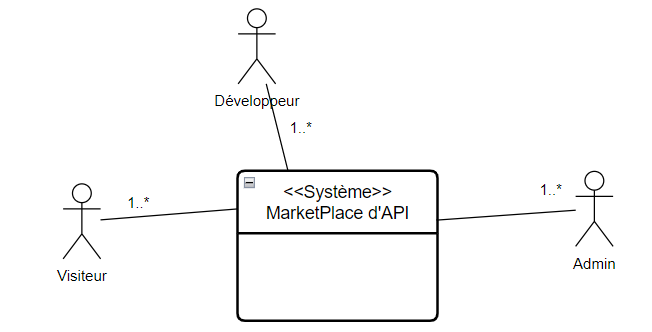
\includegraphics[width=1\columnwidth]{img/Diagramme_de_contexte_statique.png}}
        \caption{Diagramme de contexte statique }
        \label{fig:logo_tt}
    \end{figure}

\pagebreak

    \subsection{Diagramme de cas d’utilisation}
    La figure, ci-dessous, illustre le diagramme de cas d’utilisation du premier sprint sachant qu’un  utilisateur est un acteur fictif pouvant être soit un développeur, soit un administrateur. Il peut consulter les APIs et gérer son profil.
    
    \begin{figure}[H]
        \centering
        \frame{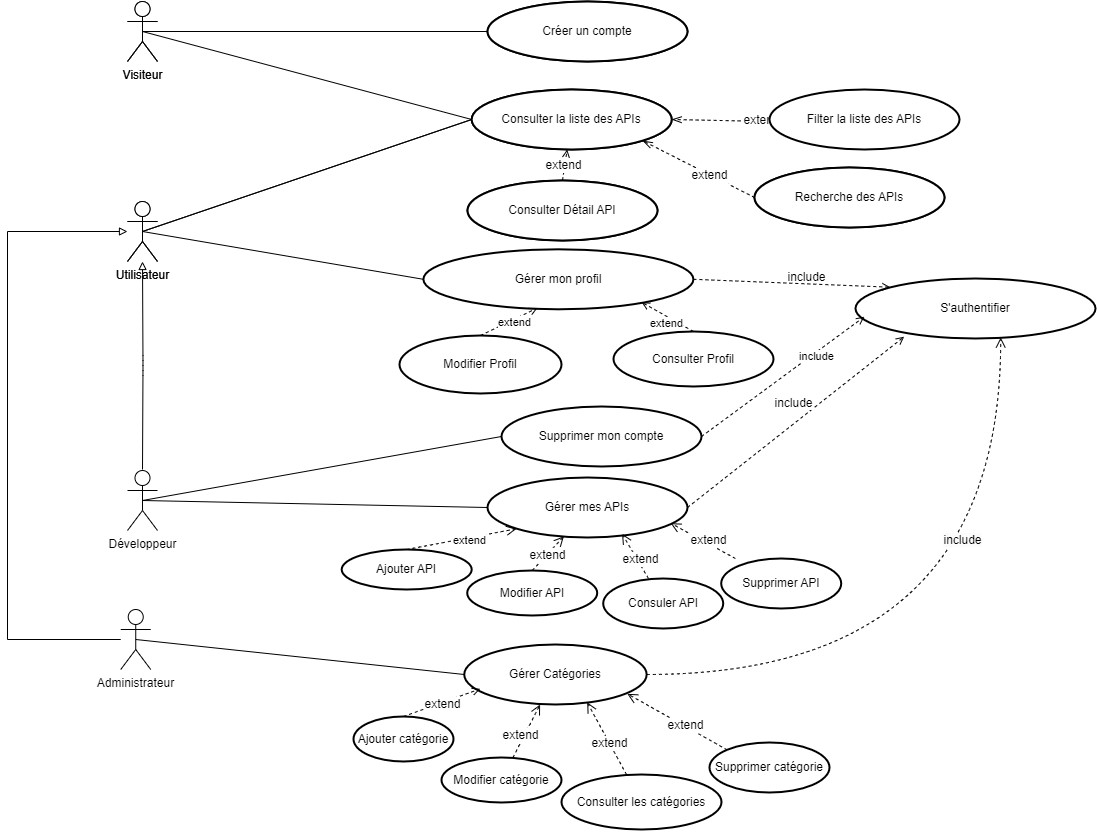
\includegraphics[width=1.1\columnwidth]{Diagramme_de_cas_d'utilisation_du_sprint_1.jpg}}
        \caption{Diagramme de cas d'utilisation du sprint 1 }
        \label{fig:logo_tt}
    \end{figure}
\pagebreak
    \subsection{Exemple d’une maquette d’interface}
    La figure suivante représente la maquette de l’interface de consultation de la liste des APIs de la marketplace  
    \begin{figure}[H]
        \centering
        \frame{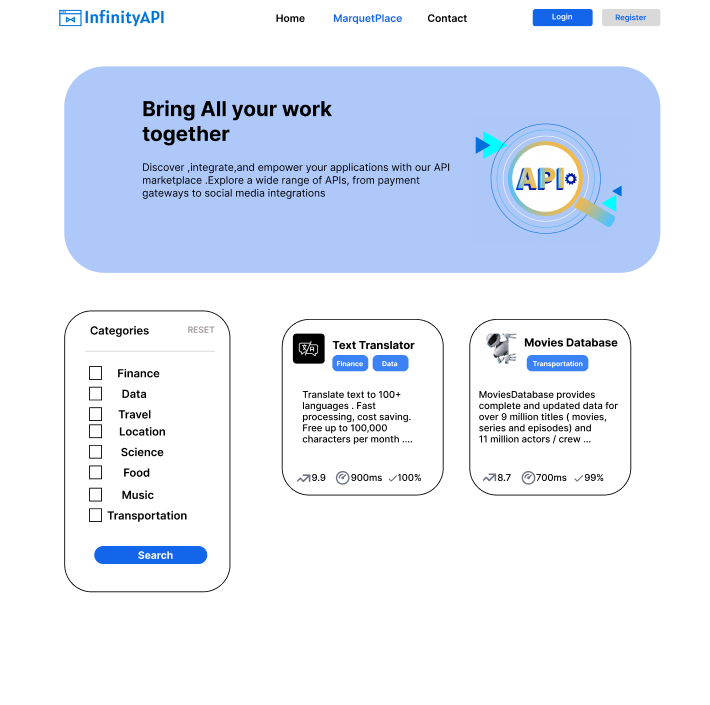
\includegraphics[width=1\columnwidth]{Maquette_de_l'interface_liste_des_APIs.png}}
        \caption{Maquette de l'interface liste des APIs }
        \label{fig:logo_tt}
    \end{figure}
\pagebreak

\section{Conception}
Dans cette partie, nous présentons le diagramme de classes, le diagramme d'activités, et enfin, les diagrammes de séquence.

    \subsection{Modélisation structurelle}

        \subsubsection{Règles de gestion}
        Voici les principales règles de gestion avant de présenter le diagramme de classes :
        \begin{itemize}
            \item  Un administrateur et un développeur sont des utilisateurs.
            \item Un développeur peut fournir zéro ou plusieurs APIs.
            \item Une API peut être fournie par un seul développeur.
            \item Une API peut appartenir à une ou plusieurs catégories.
            \item Une catégorie concerne zéro ou plusieurs APIs
        \end{itemize}

        \subsubsection{Description des principales classes}
        Notre diagramme est composé de plusieurs classes qui interagissent entre elles. Il est possible de distinguer :

        \begin{itemize}
            \item La classe “Developper” stocke les informations de base sur le développeur inscrit dans notre Marketplace telles que son nom, son prénom, le mot de passe et l'e-mail.
            \item La classe “API” stocke les informations de base sur les APIs disponibles dans le système, telles que le nom, la description et l'URL. Elle facilite la gestion et l'accès aux APIs pour les développeurs.
            \item La classe "Category" stocke les informations sur les catégories auxquelles les APIs appartiennent telles que le nom de la catégorie et une description pour aider à organiser les APIs et à faciliter la recherche et la navigation pour les utilisateurs.
        \end{itemize}
    \pagebreak

        \subsubsection{Diagramme de classes}
        Le diagramme de classes se présente comme suit :
        \begin{figure}[H]
            \centering
            \frame{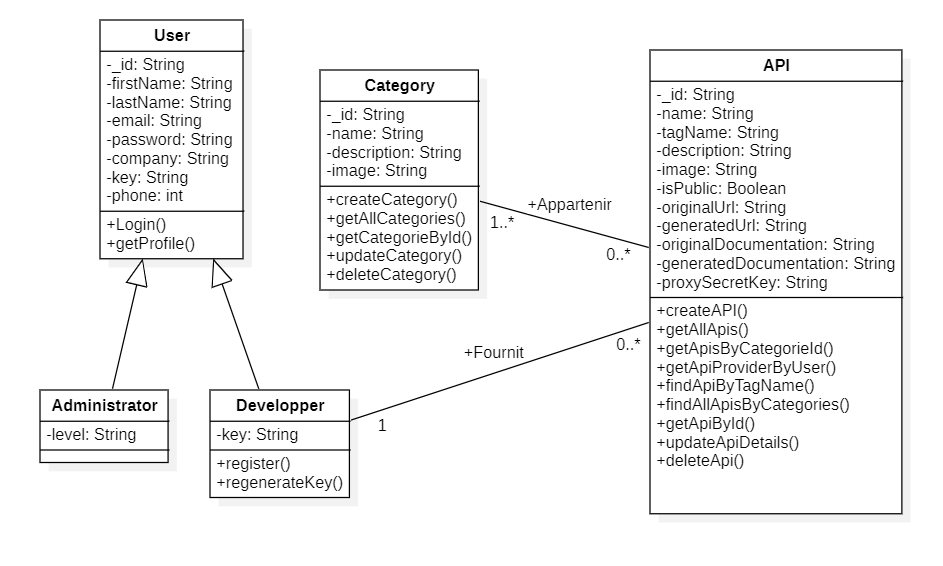
\includegraphics[width=1\columnwidth]{Diagramme_de_classe_du_sprint1.png}}
            \caption{ Diagramme de classes du sprint 1 }
            \label{fig:logo_tt}
        \end{figure}

        \subsubsection{La représentation NoSQL associée à la base de données de la MarketPlace d’API}
        Nous avons opté pour une base de données NoSQL pour notre marketplace d’API car elle s’adapte facilement aux changements, contrairement aux bases de données SQL qui sont moins flexibles. \\
        De plus, NoSQL gère mieux les grandes quantités de données complexes et assure que notre service reste disponible sans interruption, ce qui est essentiel pour répondre efficacement à la forte demande de notre plateforme dynamique.\\
        Par rapport au coût, NoSQL offre des solutions open-source disponibles sur le marché permettant de réduire considérablement les coûts de stockage et de maintenance par rapport aux bases de données SQL.\\
        Ainsi, notre base de données comporte 3 collections pour notre premier sprint. \\
    \pagebreak

        Elle se présente comme suit :
        
        \begin{figure}[H]
            \centering
            \frame{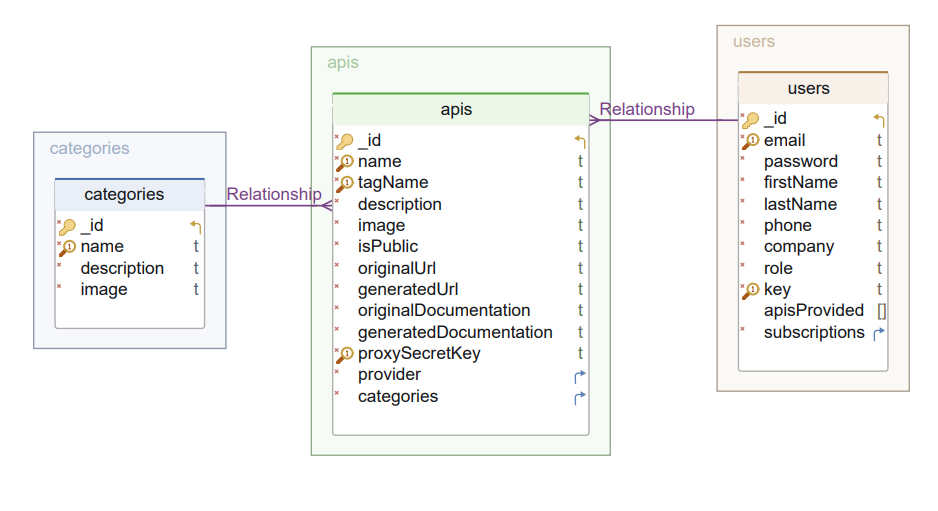
\includegraphics[width=0.8\columnwidth]{Représentation_de_la_base_de_données_du_sprint1.png}}
            \caption{ Représentation de la base de données du sprint 1 }
            \label{fig:logo_tt}
        \end{figure}

    \subsection{Diagramme d’activités "Ajouter API"}

 
    Le diagramme d’activités suivant représente le processus de création d'une API. Un développeur soumet les détails de l'API via un formulaire. Le système vérifie ensuite la validité du jeton JWT pour authentifier l'accès à la fonctionnalité de création d'API. Si le jeton est valide, le système récupère les détails de l'utilisateur et vérifie son existence. \\
    Si l'utilisateur n'existe pas, il est redirigé vers la page d'authentification. Sinon, le système vérifie la validité des détails de l'API. Il s'assure également que le nom et le tag de l'API ne sont pas déjà utilisés. Si les détails sont valides et uniques, une nouvelle URL de consommation unique est générée. Cette URL est utilisée par les consommateurs pour accéder à l'API et à ses fonctionnalités. L'URL est générée à l'aide d'un algorithme qui garantit qu'elle est unique et sécurisée. \\
    Le système vérifie ensuite le chargement correct du fichier Swagger/OpenAPI de documentation. Si le fichier n'est pas correctement chargé, un message d'erreur est affiché. Sinon, la documentation est sauvegardée et validée. La documentation Swagger/OpenAPI est ensuite analysée et mise à jour en fonction de la version du fichier. La nouvelle documentation est ensuite sauvegardée. \\
    Après la génération de la clé secrète unique pour l'API, celle-ci est associée de manière sécurisée à l'API dans la base de données, ce qui constitue une couche supplémentaire de sécurité, assurant que seules les requêtes munies de cette clé secrète peuvent interagir avec l'API. \\
    Enfin, tous les détails de l'API sont enregistrés dans la base de données et un message de succès est affiché. \\

    \begin{figure}[H]
        \centering
        \frame{\includegraphics[width=0.95\columnwidth]{Diagramme_d'activités_Ajouter_API.jpg}}
        \caption{ Diagramme d'activités "Ajouter API"}
        \label{fig:logo_tt}
    \end{figure}

    \subsection{Diagrammes de séquence}

    \subsubsection{Diagramme de séquence "Ajouter API"}

    Le diagramme de séquence décrit le processus de création d'une API. 
    Le développeur soumet une demande via l'interface "API\_Create". Le contrôleur "APIcreate" valide les champs soumis et utilise le service Angular "API" pour envoyer les requêtes au backend. Le middleware "middlewareAuth" vérifie les jetons d'authentification. Le contrôleur du backend "API" orchestre la création de l'API en utilisant les modèles "API" et "User". Une fois l'API est créée, une réponse est renvoyée au service du front pour affichage.
    
    \begin{figure}[H]
        \centering
        \frame{\includegraphics[width=1.1\columnwidth]{  Diagramme_de_séquence_de_conception_AjouterAPI.jpg }}
        \caption{   Diagramme de séquence de conception "Ajouter une API"
        }
        \label{fig:logo_tt}
    \end{figure}
    \pagebreak

\subsection{Diagramme de séquence "Ajouter une catégorie"}
Ce diagramme de séquence illustre la séquence d'interactions entre les différents composants de la marketplace pour ajouter une catégorie. L'administrateur remplit le formulaire d'ajout d'une catégorie. Si les champs sont invalides, un message d'erreur est affiché. Sinon, une requête HTTP est envoyée au backend. Le backend vérifie alors la validité du jeton. Si le jeton est invalide, un message d'erreur "invalid token" est renvoyé. Sinon, le backend vérifie si la catégorie existe déjà. Si tel est le cas, une interface affiche un message d'erreur "category already exists". Sinon, un message de succès est affiché pour indiquer que la catégorie a été ajoutée avec succès.
\begin{figure}[H]
    \centering
    \frame{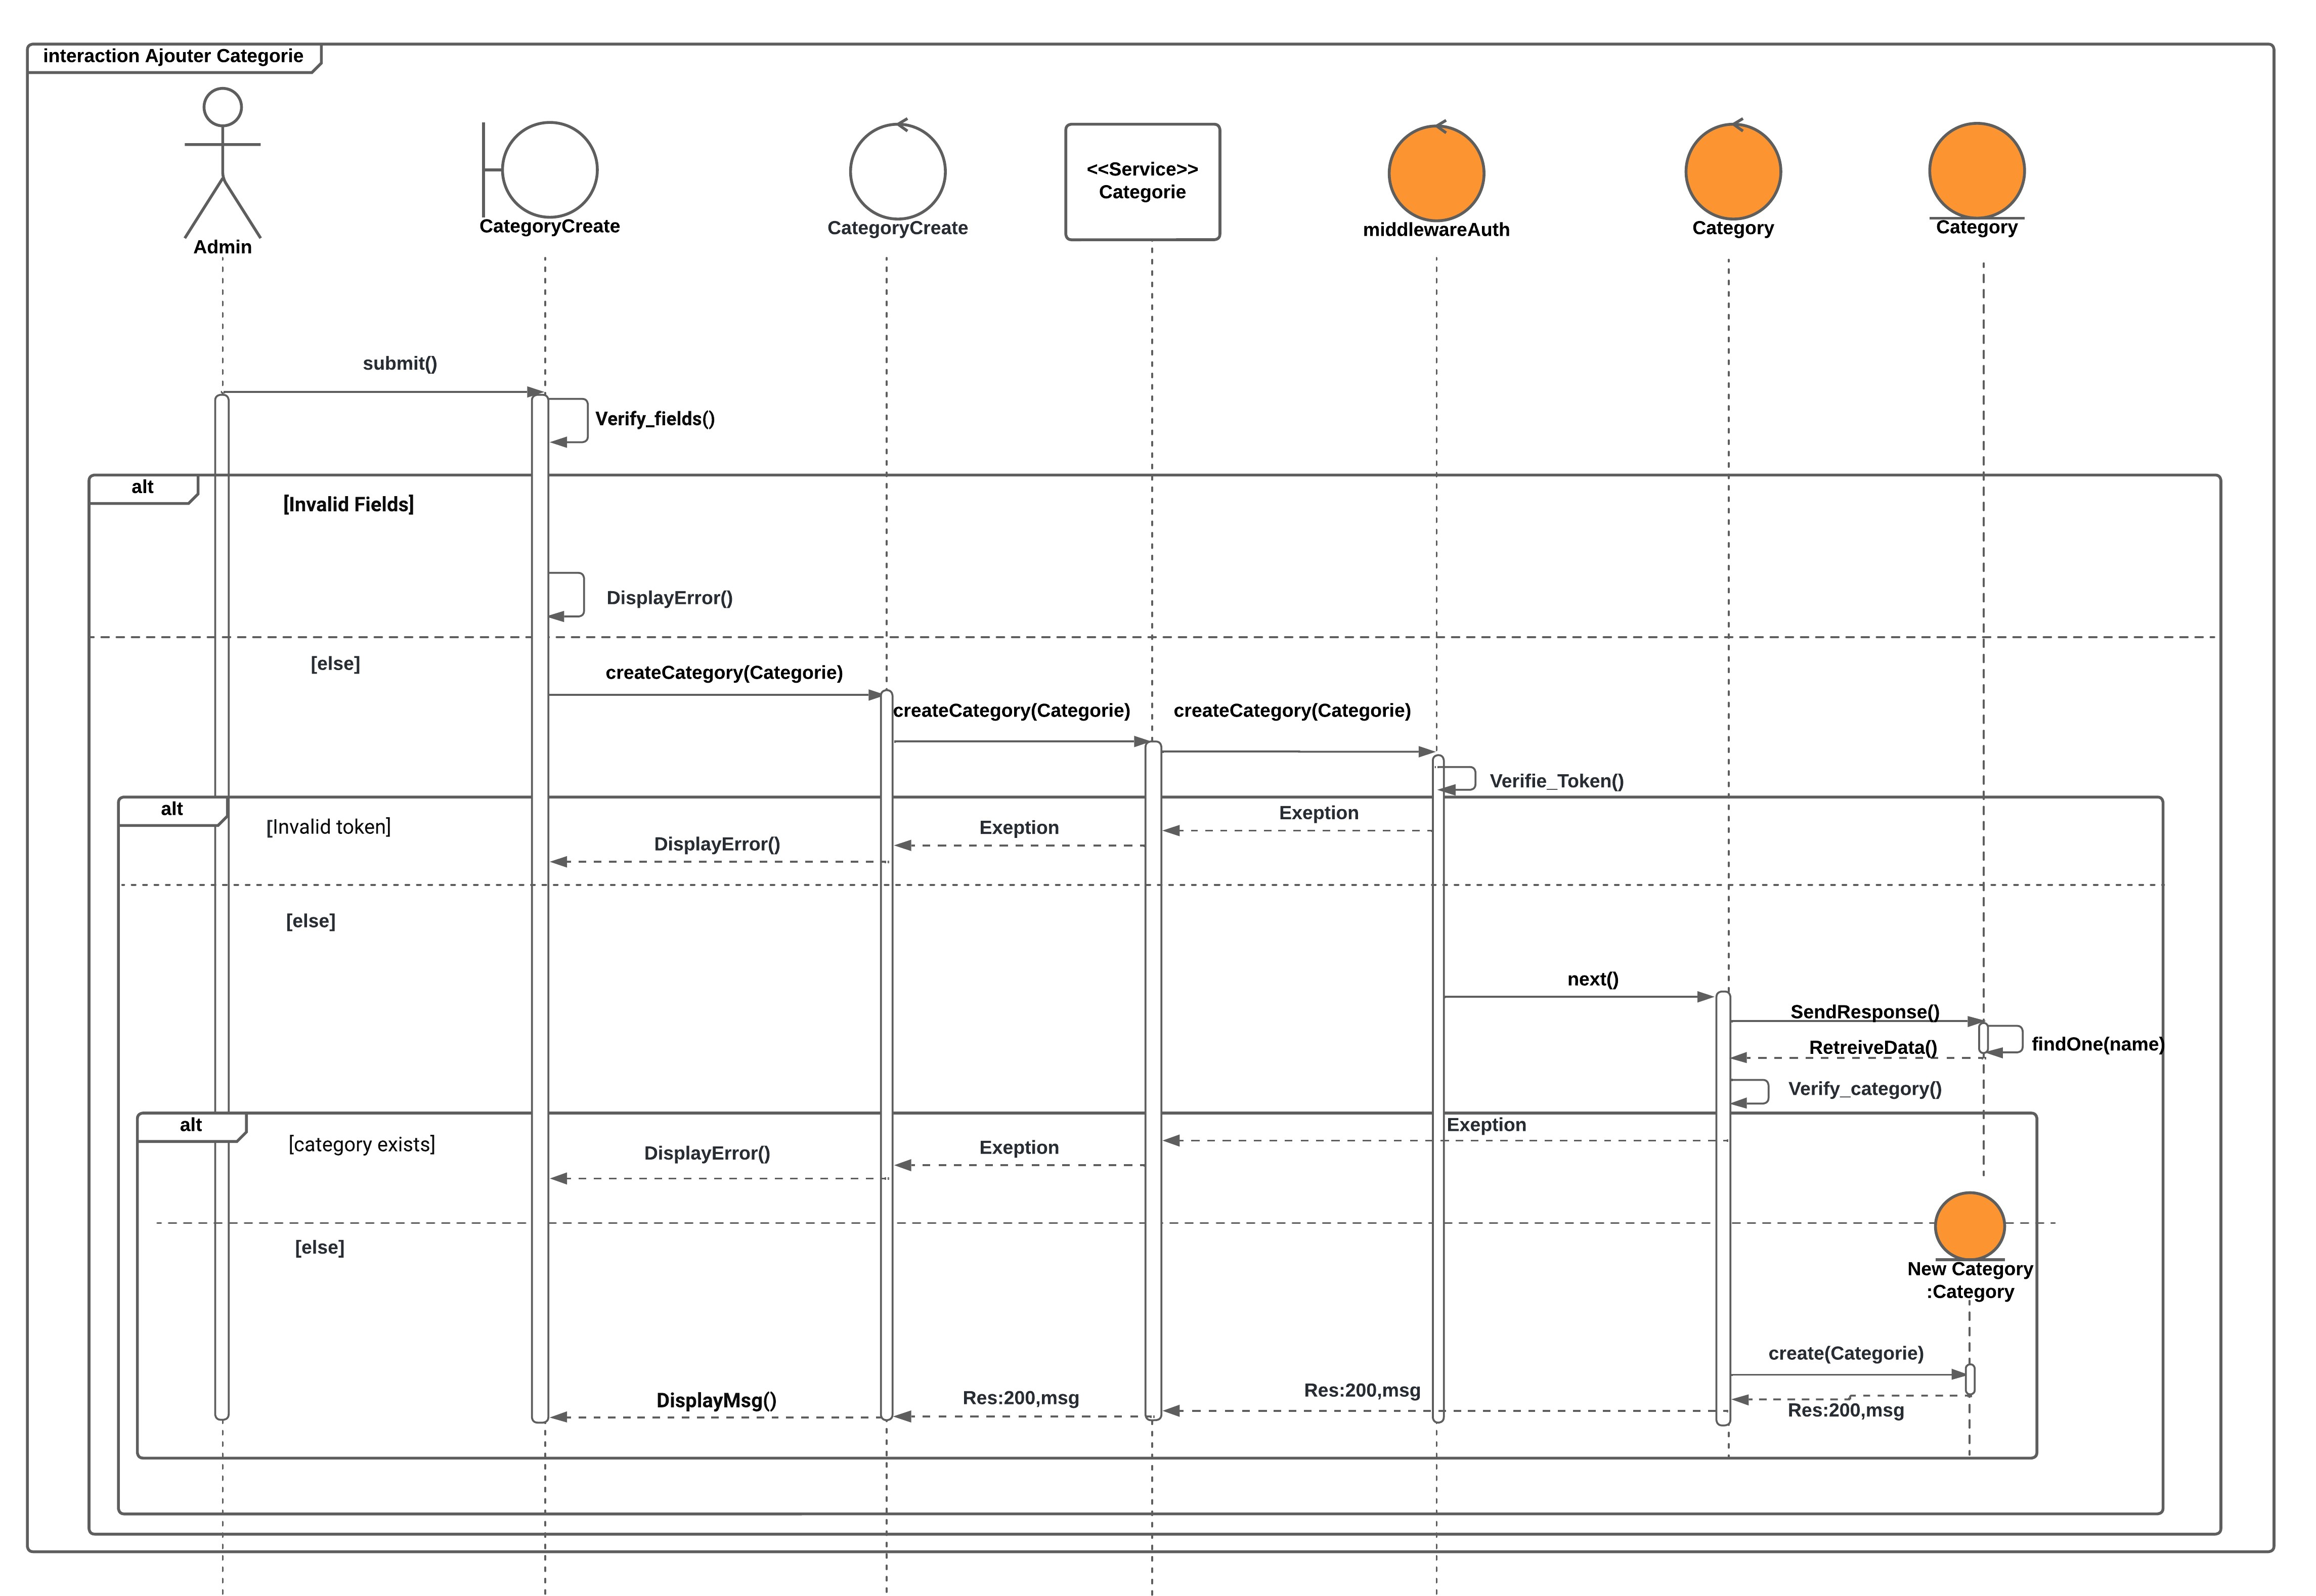
\includegraphics[width=1.1\columnwidth]{  Diagramme_de_séquence_Ajoutercatégorie.jpg}}
    \caption{ Diagramme de séquence "Ajouter une catégorie" }
    \label{fig:logo_tt}
\end{figure}
 \pagebreak



  
    \section{Revue de sprint}
    La revue du premier sprint expose le travail réalisé au niveau du sprint 1. Elle est divisée en deux parties : la réalisation et le burndown chart du projet.
    \subsection{Réalisation }
    Dans cette partie, nous allons présenter les interfaces réalisées au niveau du sprint 1.
    \subsubsection{Création du compte développeur et l'authentification}
        Cette interface présente la page de création d'un compte développeur 
        \begin{figure}[H]
            \centering
            \frame{\includegraphics[width=1\columnwidth]{Interfacedecréationdecompte.png}}
            \caption{Interface de création de compte}
            \label{fig:logo_tt}
        \end{figure}
    \pagebreak

        Cette interface présente la page d’authentification
        \begin{figure}[H]
            \centering
            \frame{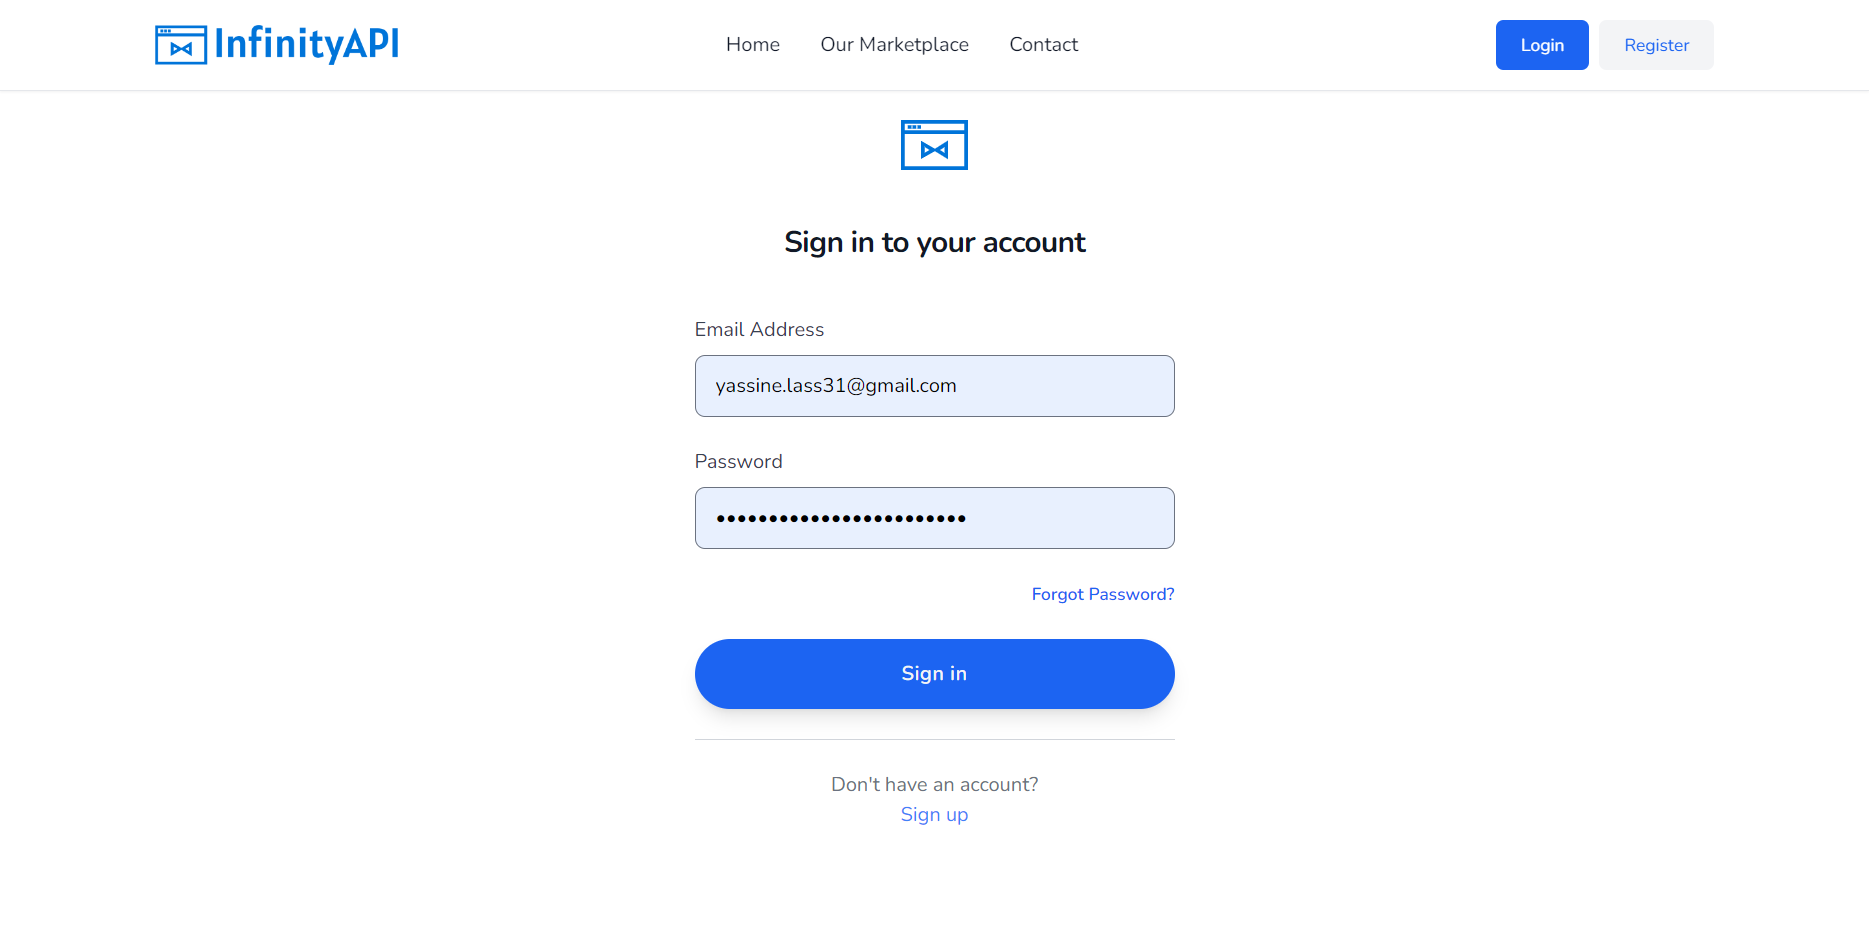
\includegraphics[width=0.8\columnwidth]{Interface_dauthentification.png}}
            \caption{Interface d'authentification}
            \label{fig:logo_tt}
        \end{figure}

    \subsubsection{Gestion des APIs  }
    Cette interface présente la page d'ajout d'une API
    \begin{figure}[H]
        \centering
        \frame{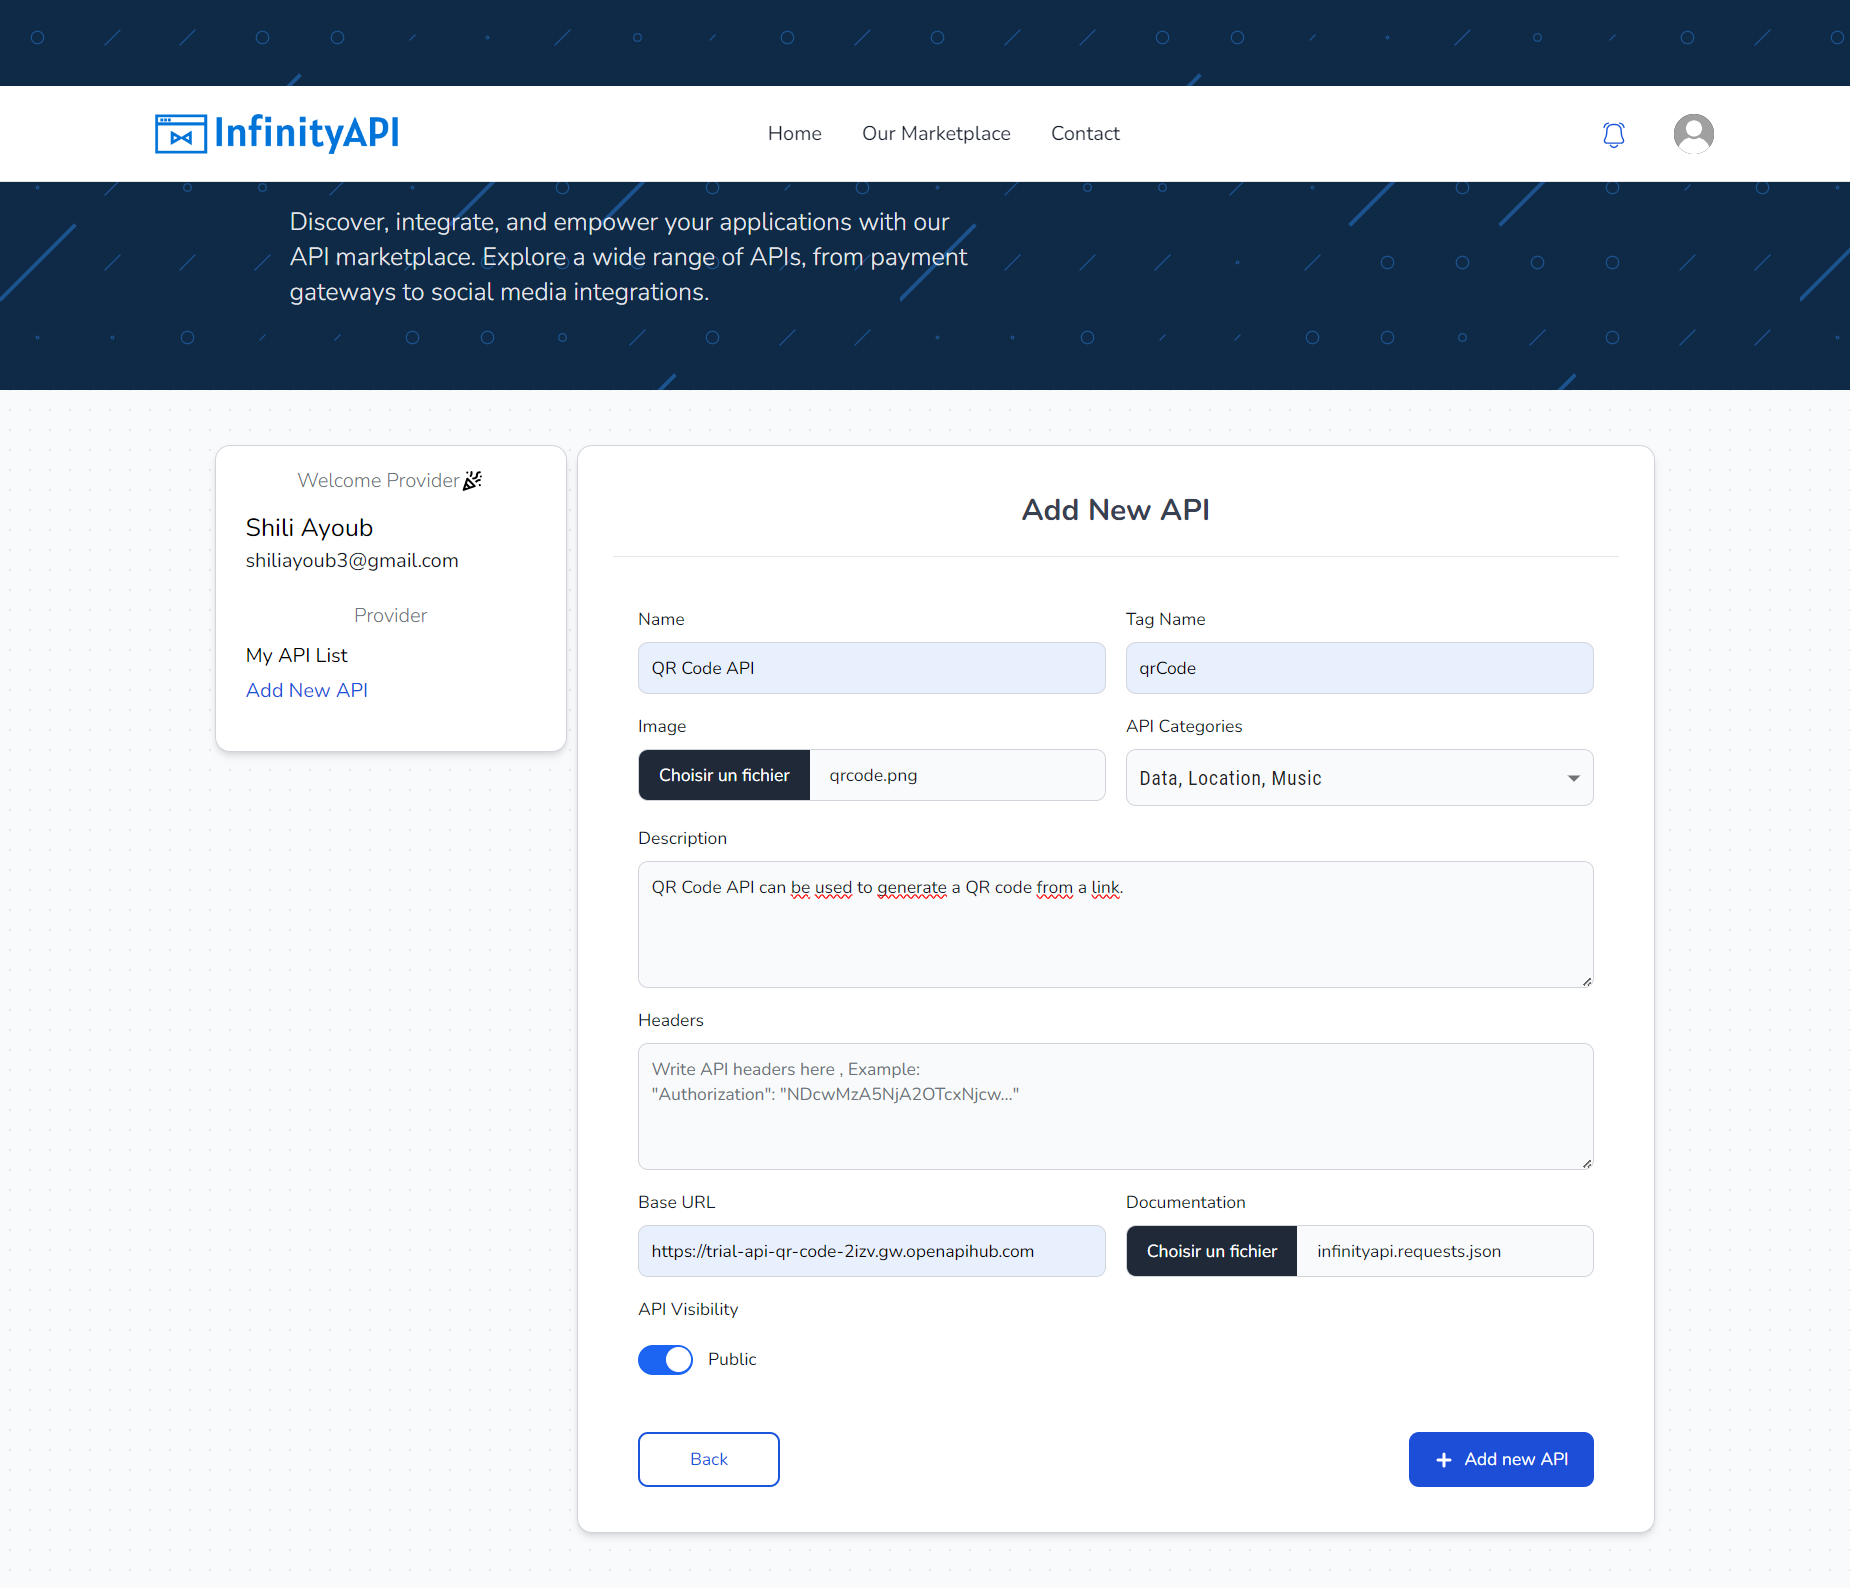
\includegraphics[width=0.85\columnwidth]{    Interface_dajout_dune_API.png        }}
        \caption{Interface d'ajout d'une API }
        \label{fig:logo_tt}
    \end{figure}
    \pagebreak


    \subsubsection{Affichage de la liste des APIs de la marketplace }	
    Cette interface présente la page de la liste des APIs consultable par le public.
    \begin{figure}[H]
        \centering
        \frame{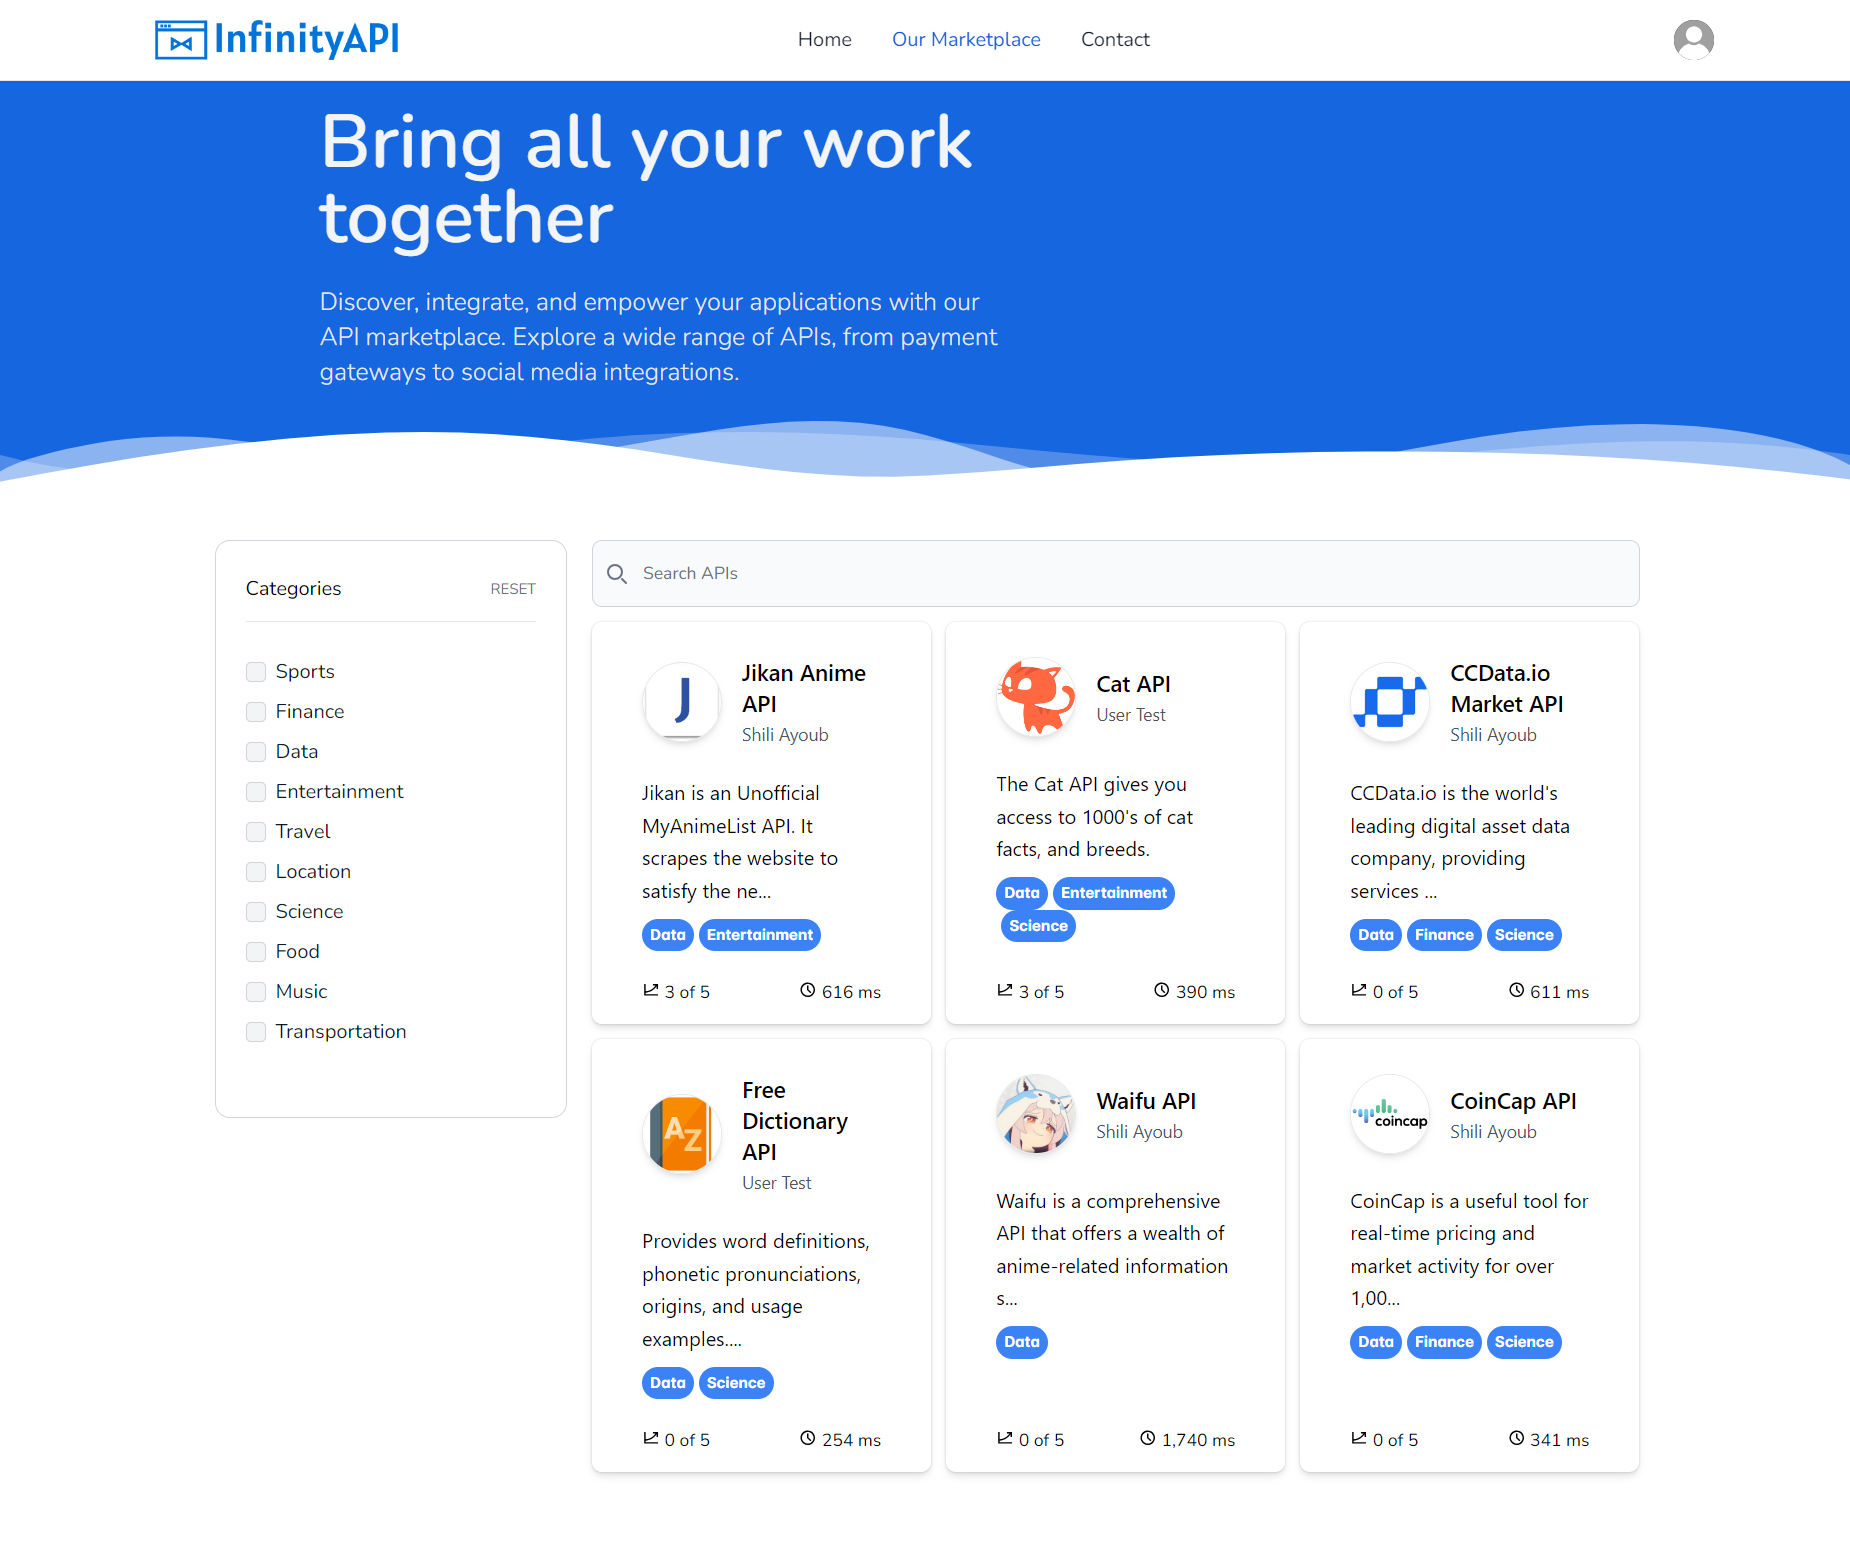
\includegraphics[width=0.7\columnwidth]{ Interface_de_liste_des_APIs.png}}
        \caption{ Interface de liste des APIs }
        \label{fig:logo_tt}
    \end{figure}
    \subsubsection{Affichage de la Documentation d'une API dans notre marketplace }	
    
    Cette interface présente la page de la documentation d'une API sélectionnée.
    \begin{figure}[H]
        \centering
        \frame{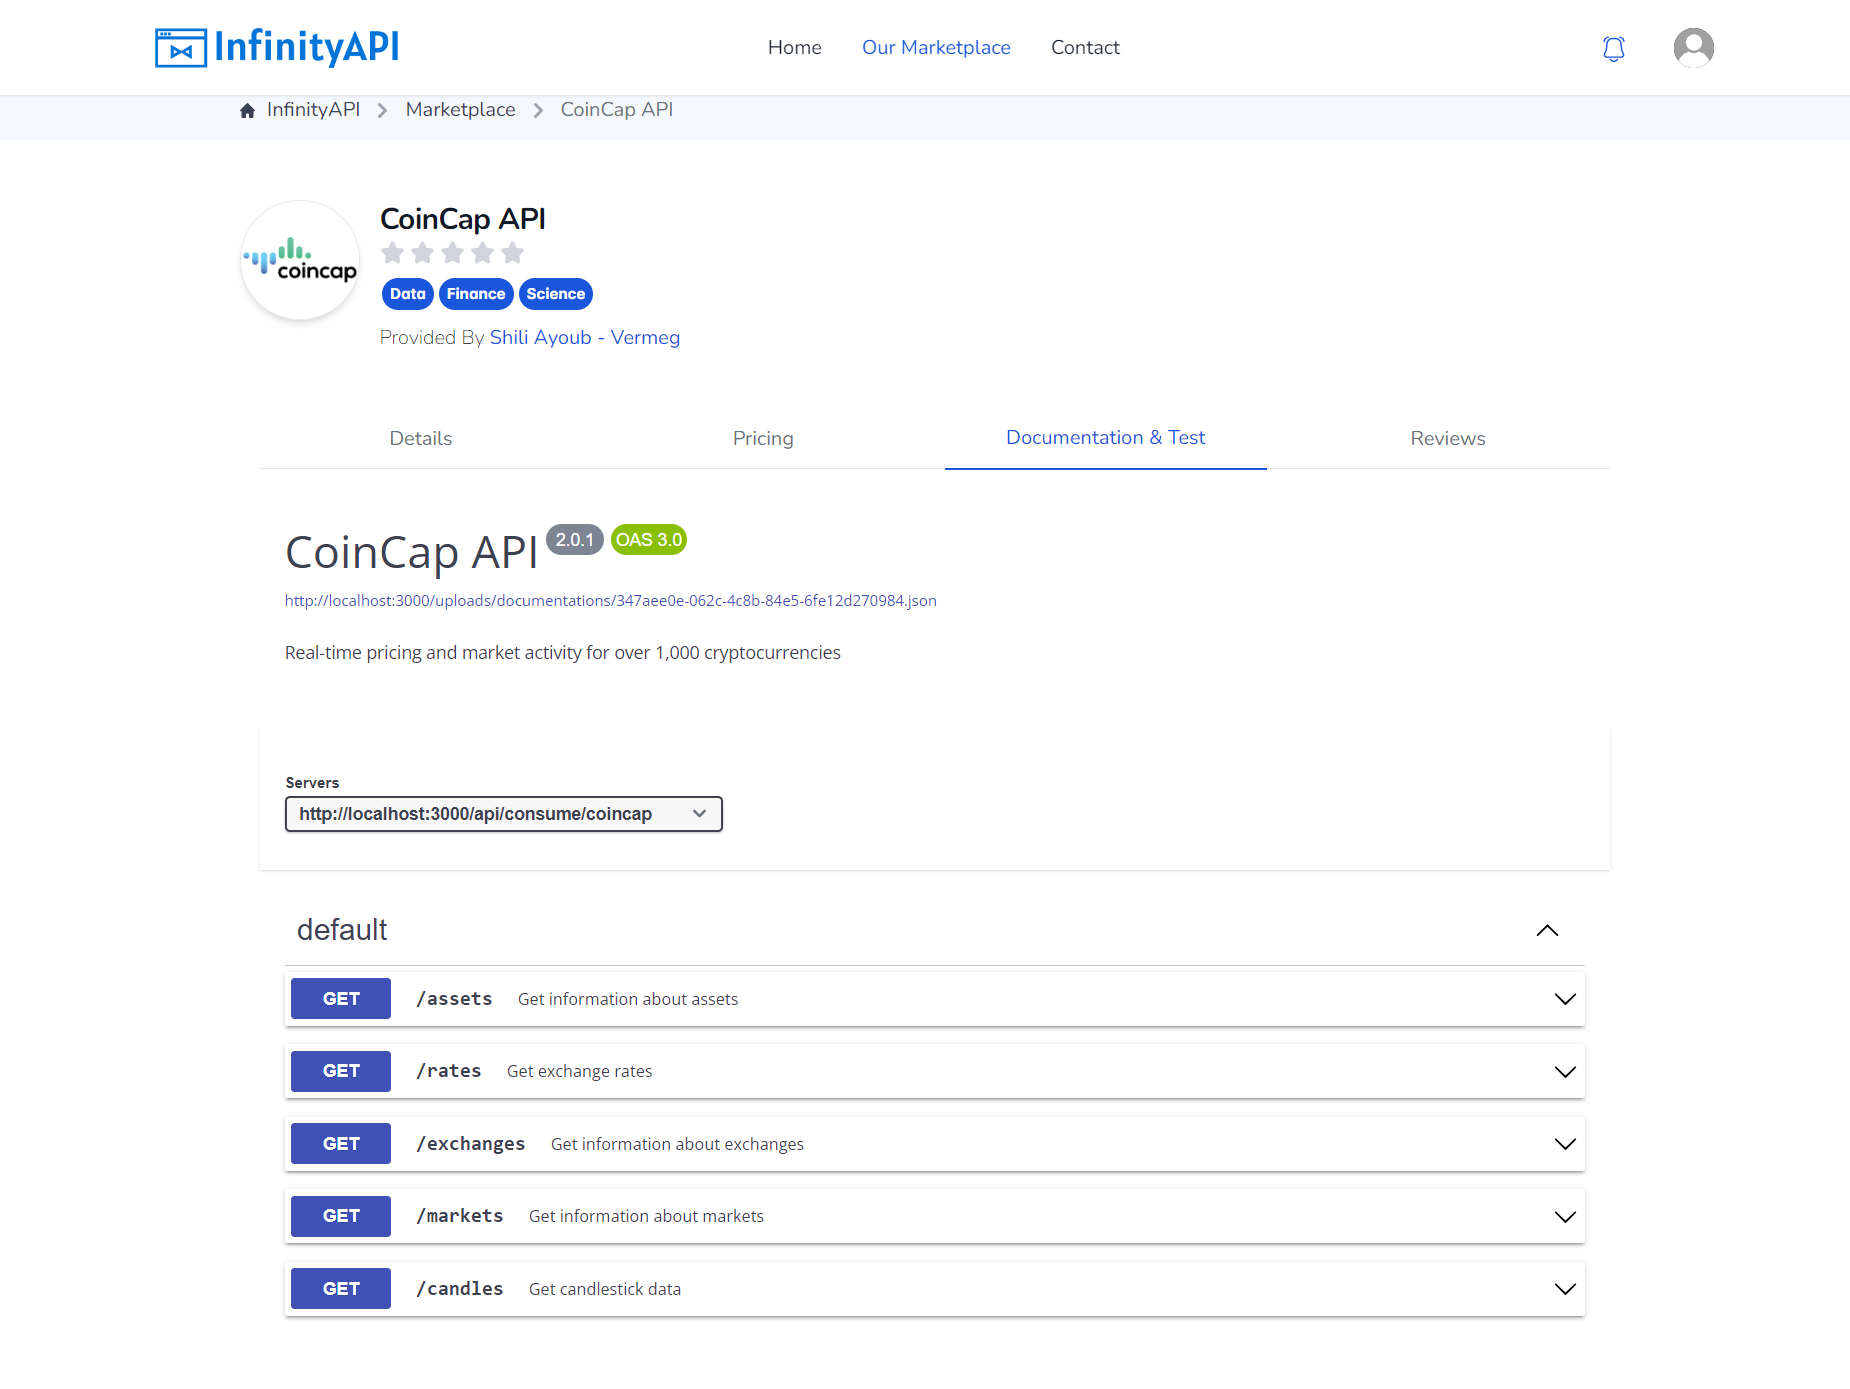
\includegraphics[width=0.7\columnwidth]{ Interface_de_test_de_lAPI.png}}
        \caption{Interface de documentation des endpoints}
        \label{fig:logo_tt}
    \end{figure}
    \pagebreak

    \subsubsection{Gestion du profil utilisateur}	
	Cette interface représente l'interface de gestion du profil développeur.
    \begin{figure}[H]
        \centering
        \frame{\includegraphics[width=0.8\columnwidth]{Interface_de_gestion_du_profil_développeur.png}}
        \caption{Interface de gestion du profil développeur}
        \label{fig:logo_tt}
    \end{figure}  
        Cette interface représente l'interface de gestion du profil administrateur.
        \begin{figure}[H]
            \centering
            \frame{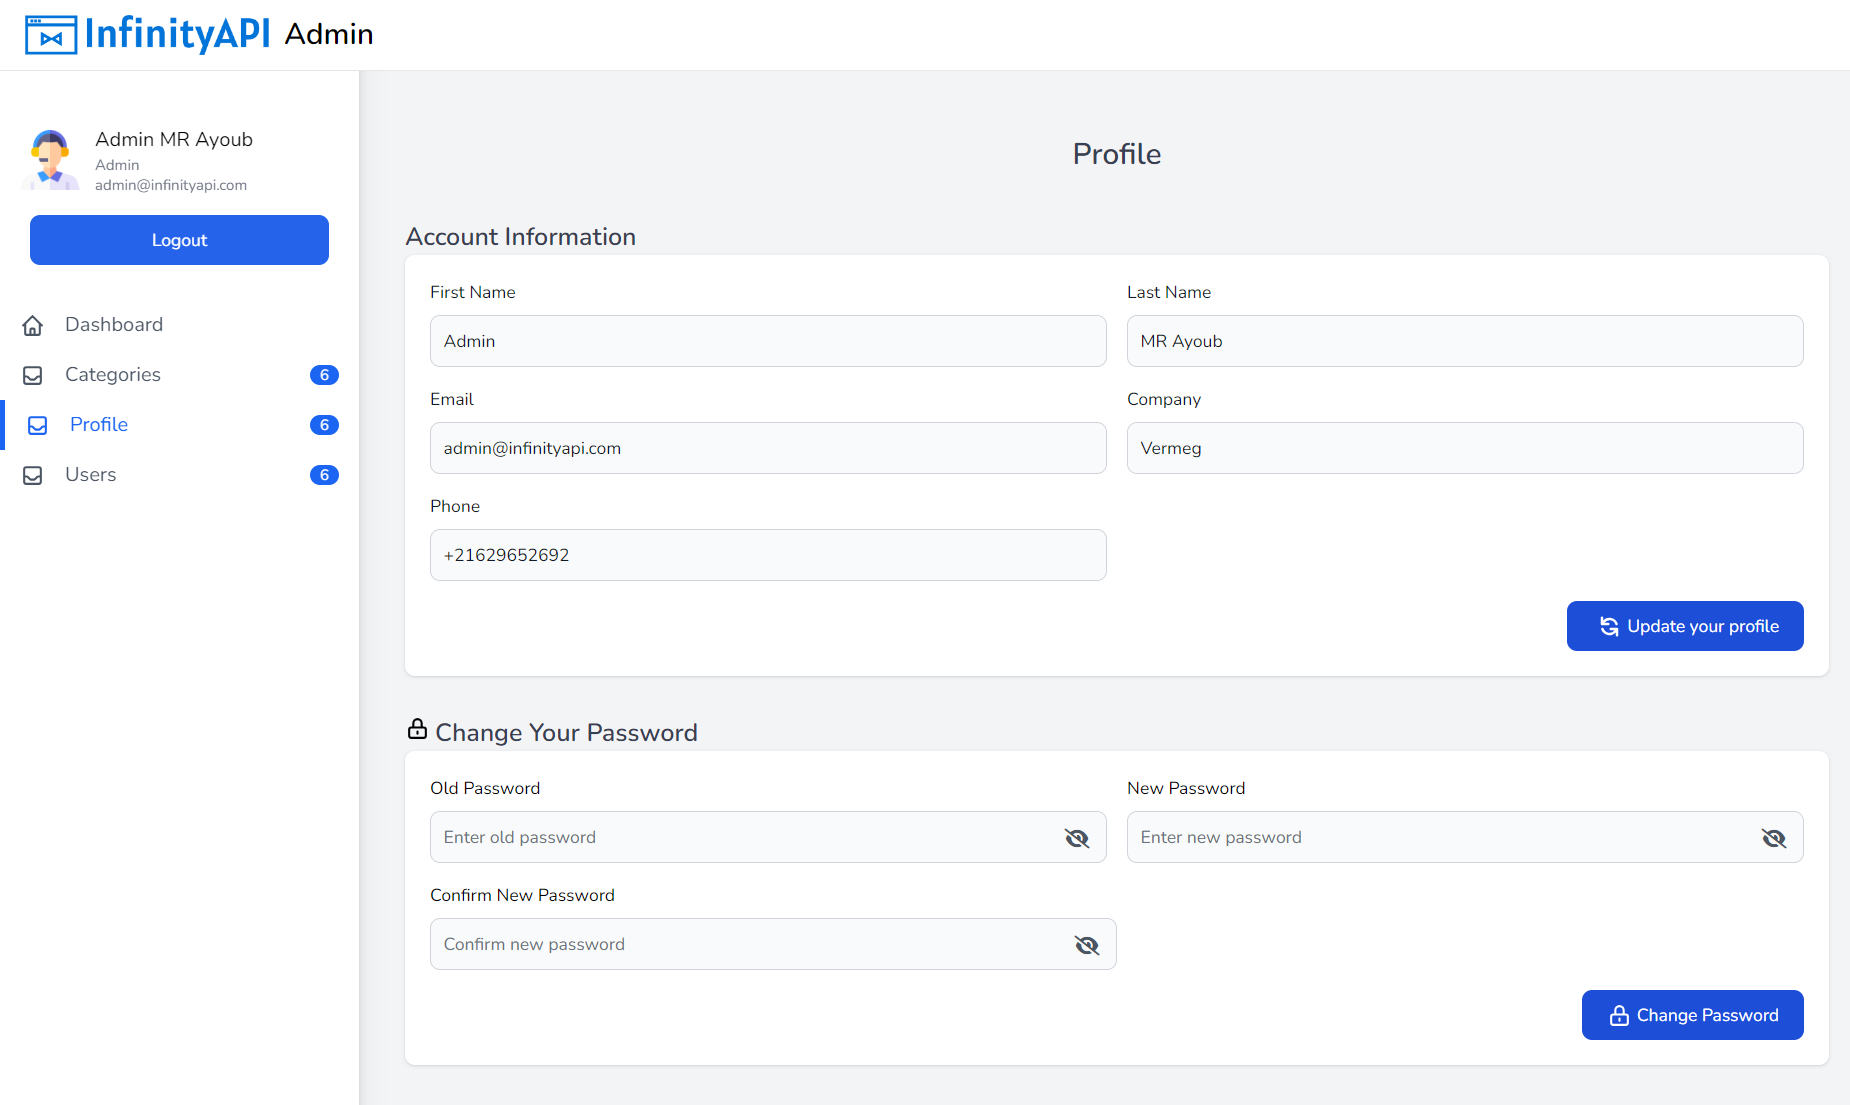
\includegraphics[width=0.8\columnwidth]{Interface_de_gestion_du_profil_administrateur.png}}
            \caption{Interface de gestion du profil d'un administrateur}
            \label{fig:logo_tt}
        \end{figure}

        \subsection{Burndown Chart}	               
        Le burndown chart va nous permettre de suivre la progression d'un projet. Il montre la quantité de travail restant (en terme d'effort estimé) par rapport au temps écoulé comme la montre la figure ci-dessous :
        \begin{figure}[H]
            \centering
            \frame{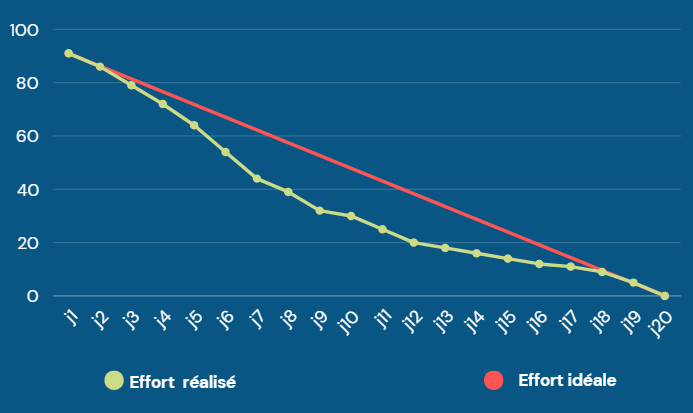
\includegraphics[width=0.9\columnwidth]{Burndown_Chart_du_sprint1.png}}
            \caption{Burndown Chart du sprint 1}
            \label{fig:logo_tt}
        \end{figure}
        
        La courbe présentée indique que nous n'avons pas correctement estimé les efforts des user stories. \\
        La vélocité de notre équipe est évaluée à 91.

        \subsection{     Rétrospective du sprint 1        }	               
        Le tableau, ci-dessous, résume la rétrospective du premier sprint

        
        \begin{longtable}[c]{|p{0.25\linewidth}|p{0.6\linewidth}|}
            \hline
            \textbf{Les questions} & \textbf{Les réponses} \\
            \hline
            \endfirsthead
            \multicolumn{2}{c}%
            {{\bfseries \tablename\ \thetable{} -- suite de la page précédente}} \\
            \hline
            \textbf{Les questions} & \textbf{Les réponses} \\
            \hline
            \endhead
            \hline \multicolumn{2}{|r|}{{\bfseries Suite à la page suivante}} \\
            \hline
            \endfoot
            \hline
            \endlastfoot
        
            \multirow{2}{=}{Ce qui s'est bien passé} & Maîtrise des langages et des logiciels utilisés. \\
            & Achèvement des thèmes \\
            \hline
            Les problèmes rencontrés & Manque d'informations et difficulté concernant l'intégration des APIs dans notre projet. \\
            \hline
            Les choses à améliorer & Mieux organiser les tâches à faire entre nous. \\
            \hline
        \end{longtable}
 
\section*{Conclusion}
Dans ce chapitre, nous avons présenté la partie spécification fonctionnelle, conception, ainsi que la revue et la rétrospective du premier sprint. Le deuxième sprint est abordé dans le chapitre suivant.

